\documentclass[final]{beamer}
\usepackage[
  orientation=portrait,
  size=a0,
  scale=1.0
]{beamerposter}
\usepackage{lipsum}
\input{packages.tex}
\newcommand{\methodName}{Clustering Agent Representation\xspace}
\newcommand{\methodeAcronym}{CAR\xspace}
\newcommand{\reinforcementLearningAcronym}{RL\xspace}
\newcommand{\latentSpaceAcronym}{LS\xspace}
\newcommand{\neuralNetworkAcronym}{NN\xspace}
\newcommand{\explainableReinforcementLearningAcronym}{XRL\xspace}
\newcommand{\deepClusteringAcronym}{DC\xspace}
\newcommand{\plural}[1]{#1\unskip s}
\newcommand{\emphasize}[1]{\textbf{#1}}

\newcommand{\BehaviorReconstructionName}{\textit{Behavior Reconstruction}\xspace}
\newcommand{\ClusteringUniversalityName}{\textit{Clustering Universality}\xspace}
\newcommand{\AbstractionScoreName}{\textit{Abstraction Score}\xspace}

\newcommand{\AdjustedRandIndexAcronym}{ARI\xspace}

\newcommand{\OriginalPolicy}{\textcolor{mygreen}{\pi}}
\newcommand{\SurrogatePolicy}[1]{\textcolor{myred}{\pi'_{#1}}}

\newcommand{\mycomment}[2][]{
  \textcolor{red}{\textbf{[#1: #2]}}
}

\definecolor{lightgray}{gray}{0.80}
\sethlcolor{lightgray}

\colorlet{myred}{red!60!black}
\colorlet{mygreen}{green!50!black}
\colorlet{myblue}{blue!80!black}

\colorlet{myorange}{orange!80!black}
\colorlet{mypurple}{purple!80!white}

\def\numberOfSamplesToPlotCurve{50}
% define gaussian pdf
\pgfmathdeclarefunction{gauss}{3}{%
  \pgfmathparse{1/(#3*sqrt(2*pi))*exp(-((#1-#2)^2)/(2*#3^2))}%
}

\newcommand{\DisplayImgFlappyBird}[1]{%
  \includegraphics[width=0.15\textwidth, trim={1cm 2.5cm 3cm 1.25cm}, clip]{#1}%
}

\definecolor{spaceInvadersColor}{RGB}{0, 0, 255}
\newcommand{\spaceInvadersMark}{*}
\newcommand{\spaceInvadersMarkSize}{0.06cm}
\newcommand{\spaceInvadersMarkText}{
    \tikz[baseline=-0.5ex]{
      \draw[mark=\spaceInvadersMark, mark size=\spaceInvadersMarkSize, color=spaceInvadersColor] 
        plot coordinates {(0,0)};
    }
}

\definecolor{marioBrosColor}{RGB}{255, 0, 0}
\newcommand{\marioBrosMark}{square*}
\newcommand{\marioBrosMarkSize}{0.05cm}
\newcommand{\marioBrosMarkText}{
    \tikz[baseline=-0.5ex]{
      \draw[mark=\marioBrosMarkText, mark size=\marioBrosMarkSize, color=marioBrosColor] 
        plot coordinates {(0,0)};
    }
}

\definecolor{pongColor}{RGB}{255, 192, 203}
\newcommand{\pongMark}{x}
\newcommand{\pongMarkOptions}{ {line width=1.5pt}, {scale=1} }
\newcommand{\pongMarkSize}{0.11cm}
\newcommand{\pongMarkText}{
    \tikz[baseline=-0.5ex]{
      \draw[mark=\pongMark, mark size=\pongMarkSize, color=pongColor] 
        plot coordinates {(0,0)};
    }
}

\definecolor{breakoutColor}{RGB}{0, 127, 0}
\newcommand{\breakoutMark}{triangle*}
\newcommand{\breakoutMarkSize}{0.08cm}
\newcommand{\breakoutMarkText}{
    \tikz[baseline=-0.5ex]{
      \draw[mark=\breakoutMark, mark size=\breakoutMarkSize, color=breakoutColor] 
        plot coordinates {(0,0)};
    }
}

\definecolor{surroundColor}{RGB}{255, 165, 0}
\newcommand{\surroundMark}{diamond*}
\newcommand{\surroundMarkSize}{0.1cm}
\newcommand{\surroundMarkText}{
    \tikz[baseline=-0.5ex]{
      \draw[mark=\surroundMark, mark size=\surroundMarkSize, color=surroundColor] 
        plot coordinates {(0,0)};
    }
}


% --- Métadonnées ---
\title{Titre du Poster}
\author{Auteur A \and Auteur B \and Auteur C}
\institute{Laboratoire XYZ, Université de Somewhere}

% --- Hauteur cellule : on retire ~12% pour le bandeau titre ---
\newlength{\cellheight}
\setlength{\cellheight}{0.275\paperheight}

\begin{document}
\begin{frame}[t]

  % ===== BANDEAU TITRE =====
  \begin{beamercolorbox}[wd=\textwidth, center, sep=1cm]{title}
    {\usebeamerfont{title}\inserttitle}\\[0.5cm]
    {\large \insertauthor}\\[0.3cm]
    {\normalsize \insertinstitute}
  \end{beamercolorbox}

  \vspace{0.5cm}

  % ===== GRILLE =====
  \begin{columns}[totalwidth=\textwidth]

    % === COLONNE 1 ===
    \begin{column}{0.5\textwidth}
      \begin{block}{}
        \vbox to \cellheight{
          \vfill
          \input{figures/latent_space.tex}
          \vfill
        }
      \end{block}
      \begin{block}{}
        \vbox to \cellheight{
          \vfill
          \input{figures/clustering_agent_representation.tex}
          \vfill
        }
      \end{block}
      \begin{block}{}
        \vbox to \cellheight{
          \vfill
          \input{figures/evolution_clustering_universality.tex}
          \vfill
        }
      \end{block}
    \end{column}

    % === COLONNE 2 ===
    \begin{column}{0.5\textwidth}
      \begin{block}{}
        \vbox to \cellheight{
          \vfill
          \NewDocumentCommand{\insertImageWithLine}{m m m m m}{
    \node[draw=#5, line width=6pt, inner sep=0] (#1) at (#2,#3) {
        \includegraphics[width=2.5cm]{#4}
    };
}

\begin{figure}
    \centering
    \resizebox{0.75\textwidth}{!}{
        \begin{tikzpicture}
            \definecolor{custom_blue}{HTML}{40568d}
            \definecolor{custom_yellow}{HTML}{fee826}
            \definecolor{custom_purple}{HTML}{440053}
            \definecolor{custom_light_green}{HTML}{5eca61}
            \definecolor{custom_dark_green}{HTML}{22928d}
        
            \begin{pgfonlayer}{background}
                \node[anchor=south west,inner sep=0] (image) at (0,0) {
                    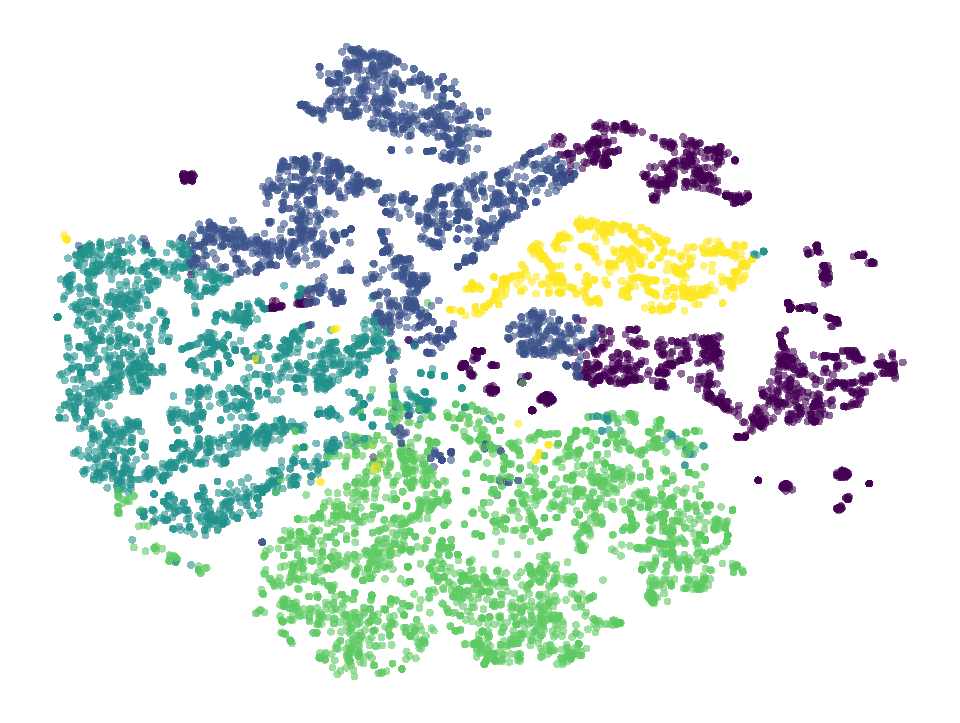
\includegraphics[]{resources/projection_2d.pdf}
                };
            \end{pgfonlayer}

            \begin{scope}[x={(image.south east)},y={(image.north west)}]
                \node[circle, draw, inner sep=0.2cm, fill=white] (cluster_1) at (0.4,0.75) {\textbf{1}};
                \insertImageWithLine{image_1}{0.17}{0.85}{pictures/space_invaders/5_clusters/early_game/image_1.png}{custom_blue}
                \insertImageWithLine{image_1}{0.35}{0.95}{pictures/space_invaders/5_clusters/early_game/image_2.png}{custom_blue}

                \node[circle, draw, inner sep=0.2cm, fill=white] (cluster_2) at (0.65,0.63) {\textbf{2}};
                \insertImageWithLine{image_1}{0.57}{0.85}{pictures/space_invaders/5_clusters/finish_right_group/image_1.png}{custom_yellow}
                \insertImageWithLine{image_1}{0.75}{0.85}{pictures/space_invaders/5_clusters/finish_right_group/image_2.png}{custom_yellow}
                
                \node[circle, draw, inner sep=0.2cm, fill=white] (cluster_3) at (0.775,0.50) {\textbf{3}};
                \insertImageWithLine{image_1}{0.9}{0.55}{pictures/space_invaders/5_clusters/catch_flying_saucer/image_1.png}{custom_purple}
                \insertImageWithLine{image_1}{0.85}{0.25}{pictures/space_invaders/5_clusters/catch_flying_saucer/image_2.png}{custom_purple}

                \node[circle, draw, inner sep=0.2cm, fill=white] (cluster_4) at (0.525,0.25) {\textbf{4}};
                \insertImageWithLine{image_1}{0.65}{0.125}{pictures/space_invaders/5_clusters/late_game/image_1.png}{custom_light_green}
                \insertImageWithLine{image_1}{0.40}{0.125}{pictures/space_invaders/5_clusters/late_game/image_2.png}{custom_light_green}

                \node[circle, draw, inner sep=0.2cm, fill=white] (cluster_5) at (0.25,0.45) {\textbf{5}};
                \insertImageWithLine{image_1}{0.075}{0.50}{pictures/space_invaders/5_clusters/mid_game/image_1.png}{custom_dark_green}
                \insertImageWithLine{image_1}{0.175}{0.20}{pictures/space_invaders/5_clusters/mid_game/image_2.png}{custom_dark_green}
            \end{scope}
        \end{tikzpicture}
    }
\end{figure}
          \vfill
        }
      \end{block}
      \begin{block}{}
        \vbox to \cellheight{
          \vfill
          \input{figures/clustering_universality.tex}
          \vfill
        }
      \end{block}
      \begin{block}{}
        \vbox to \cellheight{
          \vfill
          \begin{figure}
    \centering
    \resizebox{0.80\textwidth}{!}{
    \begin{tikzpicture}

    % ==============================
    % Partie A (2 clusters)
    % ==============================
    \node at (0, 2cm) {\textbf{The case with 2 clusters.}};

    \node (ligne_1) at (0, 0) {};

    \node[] at ($(ligne_1) + (-3.5cm, 0cm)$) {
    \begin{minipage}{8.5cm}
        \centering
        \begin{tikzpicture}
            % Première image
            \node[anchor=south west,inner sep=0] (image1) at (0,0) {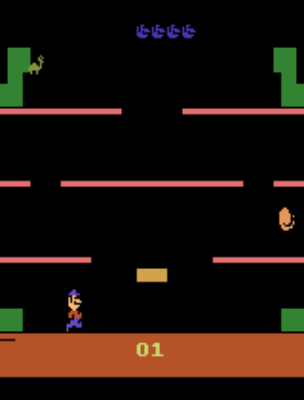
\includegraphics[width=2cm]{pictures/mario_bros/2_clusters/bloc_pow_available/image_1.png}};
            \begin{scope}[shift={(image1.south west)}, x={(image1.south east)}, y={(image1.north west)}]
                \draw[red, line width=1pt] (0.4,0.275) rectangle (0.6,0.355);
            \end{scope}
            
            % Deuxième image
            \node[anchor=south west,inner sep=0] (image2) at (image1.south east) [xshift=0.05cm] {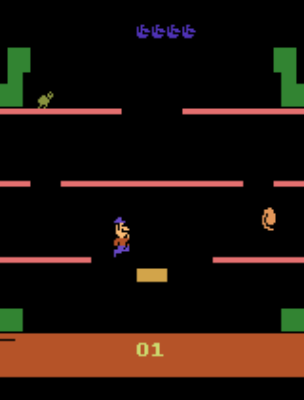
\includegraphics[width=2cm]{pictures/mario_bros/2_clusters/bloc_pow_available/image_2.png}};
            \begin{scope}[shift={(image2.south west)}, x={(image2.south east)}, y={(image2.north west)}]
                \draw[red, line width=1pt] (0.4,0.275) rectangle (0.6,0.355);
            \end{scope}
            
            % Troisième image
            \node[anchor=south west,inner sep=0] (image3) at (image2.south east) [xshift=0.05cm] {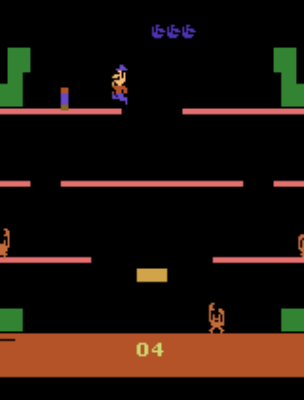
\includegraphics[width=2cm]{pictures/mario_bros/2_clusters/bloc_pow_available/image_3.png}};
            \begin{scope}[shift={(image3.south west)}, x={(image3.south east)}, y={(image3.north west)}]
                \draw[red, line width=1pt] (0.4,0.275) rectangle (0.6,0.355);
            \end{scope}
        \end{tikzpicture}
        
        \small The POW block is present.
    \end{minipage}
    };

    \node[] at ($(ligne_1) + (3.5cm, 0cm)$) {
    \begin{minipage}{8.5cm}
        \centering
        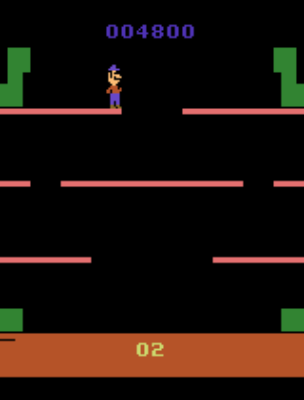
\includegraphics[width=2cm]{pictures/mario_bros/2_clusters/bloc_pow_available_not/image_1.png}
        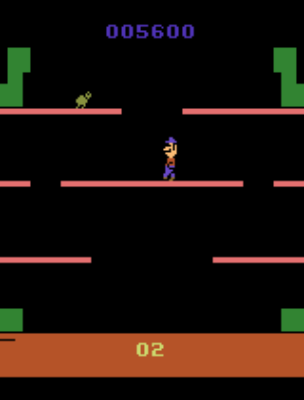
\includegraphics[width=2cm]{pictures/mario_bros/2_clusters/bloc_pow_available_not/image_2.png}
        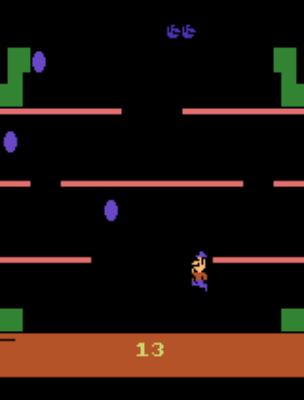
\includegraphics[width=2cm]{pictures/mario_bros/2_clusters/bloc_pow_available_not/image_3.png}
        
        \small The POW block is absent.
    \end{minipage}
    };

    % ==============================
    % Ligne de séparation
    % ==============================
    \draw[dashed, thick] (-7,-2cm) -- (7,-2cm);

    % ==============================
    % Partie B (5 clusters)
    % ==============================
    \node at (0, -2.5cm) {\textbf{The case with 5 clusters.}};

    \node (ligne_2) at (0, -4.5cm) {};

    \node[] at ($(ligne_2) + (-4.5cm, 0cm)$) {
    \begin{minipage}{4.5cm}
        \centering
        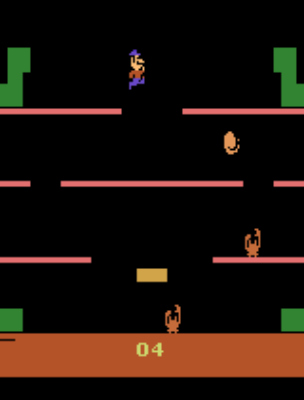
\includegraphics[width=2cm]{pictures/mario_bros/5_clusters/bloc_pow_available/image_1.png}
        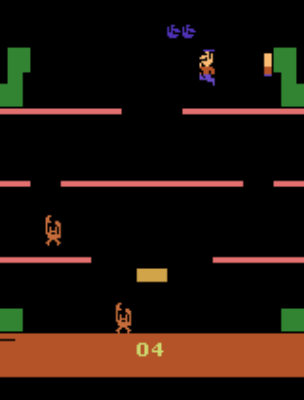
\includegraphics[width=2cm]{pictures/mario_bros/5_clusters/bloc_pow_available/image_2.png}
        
        \small The POW block is present.
    \end{minipage}
    };

    \node[] at ($(ligne_2) + (0cm, 0cm)$) {
    \begin{minipage}{4.5cm}
        \centering
        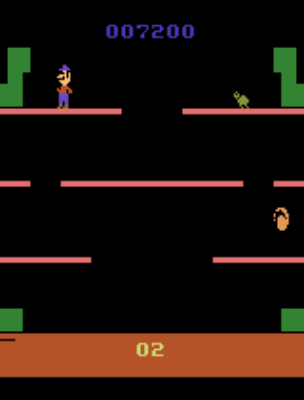
\includegraphics[width=2cm]{pictures/mario_bros/5_clusters/move_on_top_left_platform/image_1.png}
        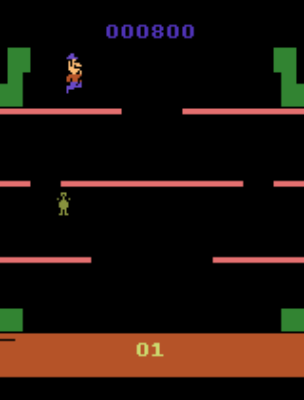
\includegraphics[width=2cm]{pictures/mario_bros/5_clusters/move_on_top_left_platform/image_3.png}
        
        \small Move on the left platform.
    \end{minipage}
    };

    \node[] at ($(ligne_2) + (4.5cm, 0cm)$) {
    \begin{minipage}{4.5cm}
        \centering
        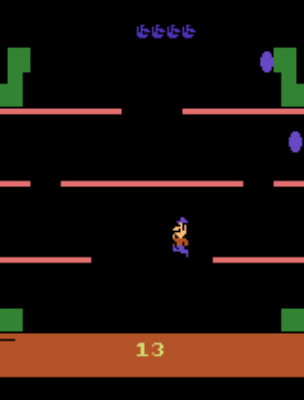
\includegraphics[width=2cm]{pictures/mario_bros/5_clusters/move_through_level/image_1.png}
        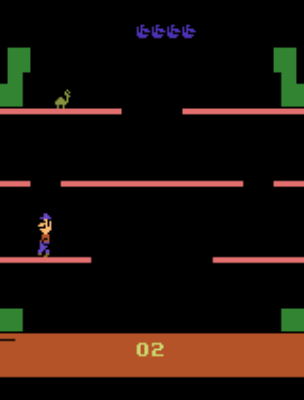
\includegraphics[width=2cm]{pictures/mario_bros/5_clusters/move_through_level/image_2.png}
        
        \small Navigating through the level.
    \end{minipage}
    };
    
    \node[] (g5) at ($(ligne_2) + (-2.25cm, -3.5cm)$) {
    \begin{minipage}{4.5cm}
        \centering
        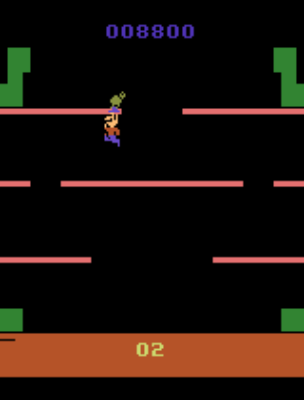
\includegraphics[width=2cm]{pictures/mario_bros/5_clusters/neutralize_enemies_left/image_1.png}
        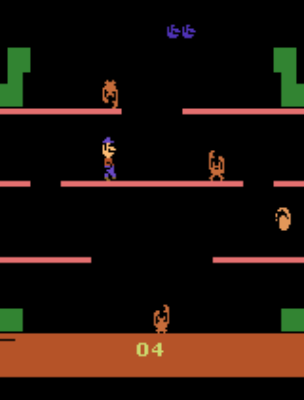
\includegraphics[width=2cm]{pictures/mario_bros/5_clusters/neutralize_enemies_left/image_3.png}
        
        \small Attacking the left.
    \end{minipage}
    };

    \node[] at ($(ligne_2) + (2.25cm, -3.5cm)$) {
    \begin{minipage}{4.5cm}
        \centering
        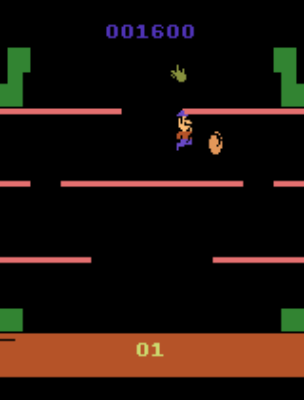
\includegraphics[width=2cm]{pictures/mario_bros/5_clusters/neutralize_enemies_right/image_1.png}
        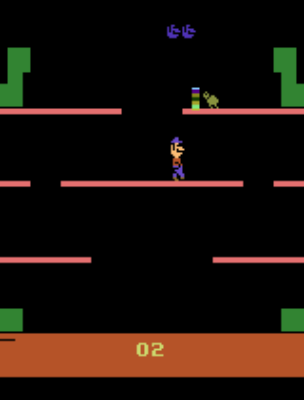
\includegraphics[width=2cm]{pictures/mario_bros/5_clusters/neutralize_enemies_right/image_2.png}
        
        \small Attacking the right.
    \end{minipage}
    };

    \end{tikzpicture}
    }
\end{figure}

          \vfill
        }
      \end{block}
    \end{column}

  \end{columns}

\end{frame}
\end{document}